\documentclass[12pt,a4paper]{article}
\usepackage[utf8]{inputenc}
\usepackage[T1]{fontenc}
\usepackage{amsmath,amssymb}
\usepackage{pgfplots}
\usepackage{tikz}
\usepackage{lmodern}
\usepackage{graphicx}
\usepackage{hyperref}
\usepackage{listings}
\usepackage{xcolor}
\usepackage{enumitem}
\usepackage{fancyhdr}
\usepackage{lastpage}
\usepackage[left=2.5cm,right=2.5cm,top=2.5cm,bottom=2.5cm]{geometry}
\usepackage[table]{xcolor}
\usepackage{array}
\usepackage{hyperref}
\usepackage{nameref}

\pagestyle{fancy}
\fancyhf{}
\renewcommand{\headrulewidth}{0pt}
\rfoot{\thepage\ af \pageref{LastPage}}

\title{Forløbsplan}
\author{Anders S. Østergaard}
\date{\today}

\definecolor{codegreen}{rgb}{0,0.6,0}
\definecolor{codegray}{rgb}{0.5,0.5,0.5}
\definecolor{codepurple}{rgb}{0.58,0,0.82}
\definecolor{backcolour}{rgb}{0.95,0.95,0.92}
\definecolor{darkerlightblue}{rgb}{0.1, 0.3, 0.5}

\lstdefinestyle{mystyle}{
	backgroundcolor=\color{backcolour},   
	commentstyle=\color{codegreen},
	keywordstyle=\color{darkerlightblue},
	numberstyle=\tiny\color{codegray},
	stringstyle=\color{codepurple},
	basicstyle=\ttfamily\footnotesize,
	breakatwhitespace=false,         
	breaklines=true,                 
	captionpos=b,                    
	keepspaces=true,                 
	numbers=left,                    
	numbersep=5pt,                  
	showspaces=false,                
	showstringspaces=false,
	showtabs=false,                  
	tabsize=2
}
\lstset{style=mystyle}
\begin{document}
	\begin{titlepage}
	\centering
	\vspace*{6cm}
	{\Huge\bfseries SWROB2\par Exam\par}
	\vspace{2cm}
	Submitted by: \par 
	\begin{table}[!h]
		\centering
		\begin{tabular}{|l|l|l|}
			\hline
			Study nr  & Name 					   & Study line\\\hline
			202005180 & Nicolaj Meldgaard Pedersen & E\\\hline
			202105443 & Johannes Baagøe 		   & E\\\hline
			201270449 & Anders Sandø Østergaard    & EP\\\hline
			201905293 & Daniel F. Borch Olsen	   & E\\\hline
		\end{tabular}
	\end{table}
	\vspace{4cm}
	Århus Universitet \par
	\vfill
	\today
\end{titlepage}
\pagenumbering{arabic}
\thispagestyle{empty}
\begin{abstract}
	\textit{This report presents the design, implementation, and evaluation of an advanced robotic system integrated with the Robot Operating System (ROS). The project leverages ROS's dynamic capabilities alongside sophisticated algorithms to enhance robotic functionalities in motion control, motion planning, perception using camera algorithms, localization, and mapping. Utilizing MATLAB and a specific hardware setup, the system demonstrates significant improvements in task efficiency and obstacle management within a controlled experimental setup. The findings highlight the system’s robustness in real-time operations and its potential for adaptation in varied automation scenarios. This study not only showcases the successful application of ROS in complex robotic tasks but also sets a foundation for future advancements in robotic automation. The report concludes with an analysis of experimental results, discussing the system's performance against predefined objectives and suggesting areas for further research.}
\end{abstract}
\clearpage
\tableofcontents
\clearpage
	\section{Kursusinformation}
	\label{sec:kursusinformation}
	\input{kursusinfo.tex}
	\section{Undervisningsforløb i Procesregulering (10 dage)}
	\input{forløb.tex}
	\clearpage
	\section{Litteratur}
	\input{litteratur.tex}
	\clearpage
	\section{Lab øvelser}
	\subsection{Opgave 1: Rockwell Skabelon}
	\label{subsec:Opgave1}
	\input{exercise5.tex}
	\subsection{Opgave 2: On/Off regulering}
	\label{subsec:Opgave2}
	\input{exercise1.tex}
	\subsection{Opgave 3: P-regulator}
	\label{subsec:Opgave3}
	\input{exercise2.tex}
	\subsection{Opgave 4: Regulering af vandtank med P-regulator og bias}
	\label{subsec:Opgave4}
	\input{exercise6.tex}
	\subsection{Opgave 5: Karakteristikker}
	\label{subsec:Opgave5}
	\input{exercise7.tex}
	\subsection{Opgave 6: Niveauregulering med PID-regulator}
	\label{subsec:Opgave6}
	\input{exercise8.tex}
	\subsection{Opgave 7: Invers/direct regulering (Ziegler \& Nichols)}
	\label{subsec:Opgave7}
	\input{exercise9.tex}
	\subsection{Opgave 8: Kaskade- og feed forward	regulering}
	\label{subsec:Opgave8}
	\input{exercise10.tex}
	\clearpage
	\section{Simuleringsøvelser}
	\subsection{Opgave 9: On/Off regulering}
	\label{subsec:Opgave1S}
	\input{exercise1S.tex}
	\subsection{Opgave 10: P-regulator}
	\label{subsec:Opgave2S}
	\input{exercise2S.tex}
%	\subsection{Opgave 11: PI-regulator}
%	\label{subsec:Opgave3S}
%	\input{exercise3S.tex}
%	\subsection{Opgave 12: PID-regulator}
%	\label{subsec:Opgave5S}
%	\input{exercise5S.tex}
%	\subsection{Opgave 13: Siemens regulator}
%	\label{subsec:Opgave6S}
%	\input{exercise6S.tex}
	\clearpage
	\section{P\&I-diagram}
	\label{sec:PIdiagram}
	\begin{figure}[h!]
		\centering
		\includegraphics[width=0.6\linewidth]{PI-diagram stand v.1.pdf}
		\caption{P\&I-diagram: Vandtank}
		\label{fig:Pidiagram}
	\end{figure}
	\section*{Symboler og Forkortelser}
	
	Nedenstående er en liste over symboler anvendt i P\&I-D for vandtanksystemet:
	\begin{table}[!h]
		\centering
		\begin{tabular}{ll}
			\textbf{Abbreviation} & \textbf{Name/Description} \\
			\hline
			LS & Level Sensor \\
			LT & Level Transmitter \\
			TT & Temperature Transmitter \\
			TCV & Temperature Control Valve \\
			FT & Flow Transmitter \\
			MV & Motor Valve \\
			FY & Flow Transmitter (Remote set) \\
			SY & Speed Control Station (Remote set) \\
			P & Pump \\
			
		\end{tabular}
	\end{table}
	\clearpage
	\section{Generel vejledning til reguleringsøvelser}
	For hver reguleringsøvelse, udarbejdes skriftlig rapport som skal indeholde og omfatte følgende:
	\begin{enumerate}
		\item PI diagram over opstillingen
		\item Blokdiagram over reguleringssløjfen
		\item Evt. kredsskema jf. Heilmann (den røde bog) fig. 4.4.6
		\item Relevante trendkurver, beskrivelser og konklusioner af forsøg.
	\end{enumerate}
	Forløbet af en øvelse, kan bygges op på følgende måde:
	\begin{itemize}
		\item [a] Optag statisk karakteristik. (regulator i manuel) Afgør om proces er med, eller uden udligning.
		\\\\
		Hvis den statiske karakteristik kan optages:
		Bedøm linearitet. Tag stilling til hvad det betyder for reguleringen. Ksløjfe = K p x Kproces = 5
		
		\item[b] Fastlæg driftspunkt, svarende til nominel belastning.
		Regulatorindstillingerne foretages omkring dette driftspunkt.
		
		\item[c] Redegør for valg af regulatorindstillingsmetode:
		\begin{itemize}
			\item[I] Ziegler Nichols (speciel for proces uden udligning) men også for øvrige processer
			\item[II] CHR og Heilmann (Proces med udligning)
		\end{itemize}

		\item[d] Regulatorindstilling ud fra valgte metoder foretages.
		
		\item[e] Afprøv først PI regulator.
		
		\item[e] Afprøv PID regulator.
	
	\end{itemize}
	Afprøvningen foretages først omkring driftspunktet, der foretages en SP ændring og/eller   belastningsændring på ca. 10 %.
	
	\begin{itemize}
		\item[g] Hvis processen ikke er lineær, gentages ovenstående afprøvning idet driftspunktet \textit{("SP")} nu hæves til ca. 90\%.
		Kommenter hvad der sker!
		
		\item[h] Resultatet af de endelige indstillinger kommenteres:
		\\\\
		Hvor godt reguleres belastnings/setpunktsændringer; PV antal oversving, \textit{("PV")}\% afvigelse fra \textit{("SP")}, tid før \textit{("PV")} ligger inden for et givet interval omkring \textit{("SP")}.
		Vurder også forløbet af \textit{("CV")}.
	\end{itemize}
	
	\clearpage
	
	\section{Opsætning af PID-regulator i Studio 5000}
	
	\textbf{Bemærk}: Kan også ses på video: Studio 5000 PID configuration
	
	\subsection*{Hovedopgave}
	\begin{itemize}
		\item ”Main Task” –> ”Properties” –> ”Configuration” –> her vælges ”Periodic” (fx. 100 mSec)
	\end{itemize}
	
	\subsection*{Analogt inputmodul}
	\begin{itemize}
		\item Analog Inputmodul ”Comm Format” skal være ”Float Data – Single-Ended Mode” (skal vælges ved første opsætning af modulet)
		\item I ”Configuration” vælges strømsignaler 4-20mA, omdannet til 0-100 (kanal 0-6), hhv. spændingssignal 0-10V, omdannet til 0-100 (kanal 7)
	\end{itemize}
	
	\subsection*{Analogt outputmodul}
	\begin{itemize}
		\item Outputmodul, ”configuration”, her vælges strømsignaler 4-20mA, omdannet fra 0-100 (kanal 0-2), hhv. spændingssignal 0-10V, omdannet fra 0-100 (kanal 3).
		\item ”Limits” i outputmodul: ”Low Clamp” og ”High Clamp” skal være hhv. 0 og 100.
	\end{itemize}
	
	\subsection*{PID-blokopsætning}
	\begin{itemize}
		\item Først skal PID-blokken navngives i taglisten.
		\item Opret en PID-blok i en rung og indtast navnet.
		\item Indsæt ”Proces Variable” (PV) analog indgang fra taglisten.
		\item Indsæt "Control Value" (CV) analog udgang fra taglisten.
		\item ”Tieback”, ”PID Master Loop”, ”Inhold Bit” og ”Inhold Value” sættes alle til 0.
	\end{itemize}
	
	\subsection*{PID Setup}
	\subsubsection*{Tuning}
	\begin{itemize}
		\item Regulatorparametrene indstilles her. Eventuelt kan f.eks. setpunkt hentes eksternt fra fx. FactoryTalckView, hvor ”Destination” sættes til tag: ”<Regulatornavn>.SP”
	\end{itemize}
	
	\subsubsection*{Configuration}
	\begin{itemize}
		\item PID Equation: ”Independent” giver separat beregning af P, I og D (ligning (3.2) i lærebog), mens ”Dependent” medfører at ændring af forstærkning også ændrer I og D (ligning (3.3) i lærebog)
		\item Control Action vælges efter om det skal være direkte (PV-SP=e) eller invers (SP-PV=e) regulering (se lærebog..)
		\item Derivative Of: bestemmer hvor D-delen af regulatoren placeres, enten i selve regulatoren sammen med P- og I-del (”error”) eller på signalet fra måleren (”PV”) (se lærebog..)
		\item Loop Update Time, skal være det samme som "Periodic time (fx. 100 mSec) og mindre end RPI for analogt inputmodul
		\item CV High Limit kan sættes til 100, men egentlig ikke nødvendigt når scaling er sat til 0-100. (Ved anvendelse af vandstande kan det være en god ide at sætte low limit til ca 25\%, da pumpen under dette omdrejningstal ikke kan overvinde modtrykket)
	\end{itemize}
	
	\subsubsection*{Scaling}
	\begin{itemize}
		\item 0-100 for PV, CV og Engineering Unit
	\end{itemize}
	
	\subsection*{Trendkurver}
	
	\begin{itemize}
		\item Højreklik på "Trends", vælg "New Trend", giv den et passende navn. I "Scope" vælges "Main Program" (eller hvor regulatoren nu er placeret), og der vælges mellem "Available Tags".
		\item Regulatorens indstillinger (SP, Kp, Ti osv.) findes under regulatorens navn (\textless{}Regulatornavn\textgreater{}.SP).
		\item Udseende, tidsakse osv. indstilles i "Properties". Bemærk at der som default er sat et begrænset antal logninger, og det vil ofte være bedst enten at øge dette, øge samplingstiden eller ændre til tidsbegrænsning – når det indtastede antal logninger nås, slettes de første data i takt med at nye logges.
		\item Bemærk at data ikke gemmes automatisk – stop logning, vælg "Log" – "Save Trend Log As". Der vil således genereres en talfil som fx. kan importeres i regneark.
	\end{itemize}
	
	\subsection*{Gem program}
	Herefter gemmes programmet, og downloades til PLC. Vær sikker på at downloade til den rigtige IP-adresse.
	\\\\
	Der kan nu eksperimenteres med forskellige indstillinger af regulatoren, hvis relevante parametre logges som Trendkurver. Signal til inputmodul kan med fordel jævnes med et digitalt filter - tidskonstanten (Tau) indstilles i "Configurations" – "Digital Filter".
	\\\\
	Regulatorparametrene kan ændres mens PLC’en kører. Efter hver ændring: tryk "Save", og vælg "Upload Tag Values", på den måde sikres at ændringer er gemt både i PLC og på PC.
	
	\clearpage
	
	\section{Statisk og dynamisk karakteristik}
	\label{sec:statiskDynamiskKarakteristik}
	\subsection*{Statisk karakteristik for systemet}
	Viser hvilken sammenhæng der er mellem indgangs- og udgangssignal. Stationær vil sige at signalerne er i ro. Dvs. den kurve man kan konstruere ud fra stationære værdier kan vises i en kurve at anvende inputsignalet på x-aksen og outputsignalet på y-aksen, vist nedenunder (der er ingen tid på x-aksen).
	
	\begin{figure}[ht]
		\centering
		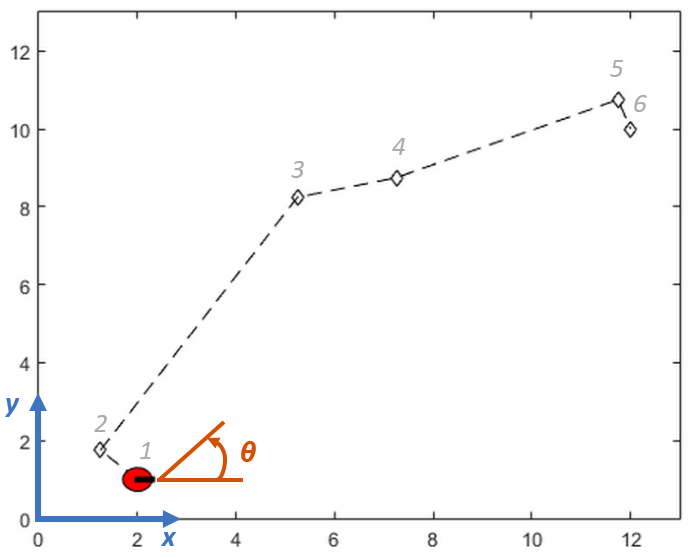
\includegraphics[width=0.5\textwidth]{fig5}
		\caption{Statisk karakteristik med input på x-aksen og output på y-aksen.}
		\label{fig:static_char}
	\end{figure}
	\noindent Hvordan gør vi her? I sætter PID regulatoren i SW manuel mode (dette kobler PID regulator ud af sløjfen, vi har en åbensløjfe), og har dermed helt styr på hvad input til systemet er. I starter med en lille inputværdi 5\% afventer et roligt stationært output, PV værdien, og noterer den. Forsøgende fortsætter indtil inputværdien når 100\%. Dermed kan de sammenhørende værdier vises i en kurve. Kurven viser forstærkningen i alle arbejdspunkter, i figuren er forstærkningen lineær.
	
	\subsection*{Dynamisk karakteristik for systemet}
	Ved den dynamiske karakteristik laves et større step på inputsignalet, og man ser på outputsignalet(PV), se figuren nedenfor. Man ser altså her på hvordan PV ændre sig over tid og identificerer dødtid, tidskonstant og beregner forstærkningen i systemet.
	\begin{figure}[ht]
		\centering
		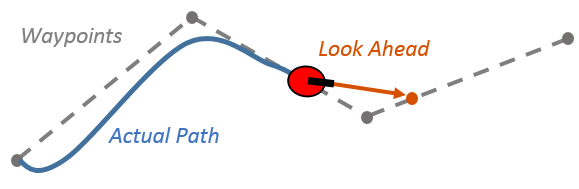
\includegraphics[width=0.5\textwidth]{fig6}
		\caption{åben sløjfe Trinrespons}
		\label{fig:trinrespons}
	\end{figure}
	
	\noindent\textbf{Tilsvarende dødtid:} Dødtiden er den periode fra trinændringen på systemets input, til du ser en begyndende ændring i output. Det er altså det tidspunkt, hvor kurven begynder at afvige fra baseline værdien. Dette kan findes ved visuel inspektion af trinresponskurven.
	\\\\
	\noindent\textbf{Tilsvarende tidskonstant:} Tidskonstanten er den tid det tager for systemet at nå 63.2\% af det nye stationære niveau efter en trinændring, efter dødtiden er udløbet. Matematisk er det tidspunktet hvor systemet har nået \(1-e^{-\frac{t}{\alpha}}\)
	(ca. 63.2\%) af den samlede ændring i output, som sker på grund af input trinændringen.
	\\\\
	\noindent\textbf{Stationær forstærkning:} 
	Steady-state Gain ($K_p$) er forholdet mellem ændringen i output ($\Delta PV$) og ændringen i input ($\Delta u$). Dette er hældningen af den linje, der passer bedst til trinresponsen, når den har nået sit nye stationære niveau
	\(K_{p} = \frac{\Delta PV}{\Delta u}\)
	\\\\
	\noindent Husk alt dette laves imens det stadigvæk er åben sløjfe at vi får det dynamiske forløb.
\end{document}